\chapter{Apéndice: Algoritmos y Ejemplos}
\label{chap:appendix}

\section{Especificación completa en \spirit}
\label{append:grammarspirit}

\lstinputlisting[basicstyle=\scriptsize, numbers=left]{input_file_code/full_grammar.cpp}

\section{Ejemplo: MAG presentada por Wuu Yang}
\label{append:agwuuyang}

\subsection{Pseudocódigo}
\begin{lstlisting}[backgroundcolor=\color{white}]
     (R1)   S `$\rightarrow$` XYZ      
              S.s0 := X.s1 + Y.s2 + Y.s3 + Z.s4
              X.i1 := Y.s3  
              Y.i2 := X.s1
              Y.i3 := Y.s2
     (R2)   Y `$\rightarrow$` m        
              Y.s2 := Y.i2
              Y.s3 := 1
     (R3)   Y `$\rightarrow$` n        
              Y.s2 := 2
              Y.s3 := Y.i3
     (R4)   X `$\rightarrow$` m        
              X.s1 := X.i1
     (R5)   Z `$\rightarrow$` Y        
              Z.s4 := Y.s3
              Y.i2 := 3
              Y.i3 := Y.s2
\end{lstlisting} 

\subsection{Con lenguaje de especificación de \maggen}

\subsubsection{Archivo de input: \textbtt{ag\_wuu\_yang.input}}
\lstinputlisting[basicstyle=\scriptsize, numbers=left, columns=fullflexible, language=specmag]{input_file_code/ag_wuu_yang.input}

\subsubsection{Archivo de output: \textbtt{Grammar\_mag.log}}
\lstinputlisting[basicstyle=\scriptsize, numbers=left, columns=fullflexible, language=specmag]{input_file_code/Grammar_mag.log}

\section{Código generado por \maggen: Ejemplo Wuu Yang.}
\label{append:agwuuyangcode}

Los archivos fueron obtenidos invocando a \maggen\ de la siguiente forma:

\begin{center}
\footnotesize{\textbtt{
maggen -fo ../Out\_wuu\_yang -o maggen -f ../examples/ag\_wuu\_yang/ag\_wuu\_yang.input
}}
\end{center}

\subsection{Archivo interface: \textbtt{maggen.hpp}}
\label{append:maggenhpp}
\lstinputlisting[basicstyle=\scriptsize, columns=fullflexible, numbers=left]{input_file_code/maggen.hpp}

\subsection{Archivo implementación: \textbtt{maggen.cpp}}
\label{append:maggencpp}
\lstinputlisting[basicstyle=\scriptsize, columns=fullflexible, numbers=left]{input_file_code/maggen.cpp}

\subsection{Archivo cabecera: \textbtt{Node.hpp}}
\label{append:nodehpp}
\lstinputlisting[basicstyle=\scriptsize, numbers=left, columns=fullflexible]{input_file_code/Node.hpp}

\subsection{Archivo cabecera: \textbtt{Plan.hpp}}
\label{append:planhpp}
\lstinputlisting[basicstyle=\scriptsize, numbers=left, columns=fullflexible]{input_file_code/Plan.hpp}

\chapter{Apéndice: Diagramas de \maggen.}
\label{append:disemaggen}
La arquitectura completa de \maggen\ se pueden visualizar en 4 capas bien definidas, con funciones y responsabilidades que fueron explicadas en los capítulos específicos de cada uno.

\begin{itemize}
\item Parsing.
\item Representación interna: GA y expresiones.
\item Construcciones de grafos, planes y secuencias de visitas.
\item Generación de código del evaluador.
\end{itemize}

Los siguientes diagramas corresponden a cada capa.

\begin{figure}[!ht]\centering
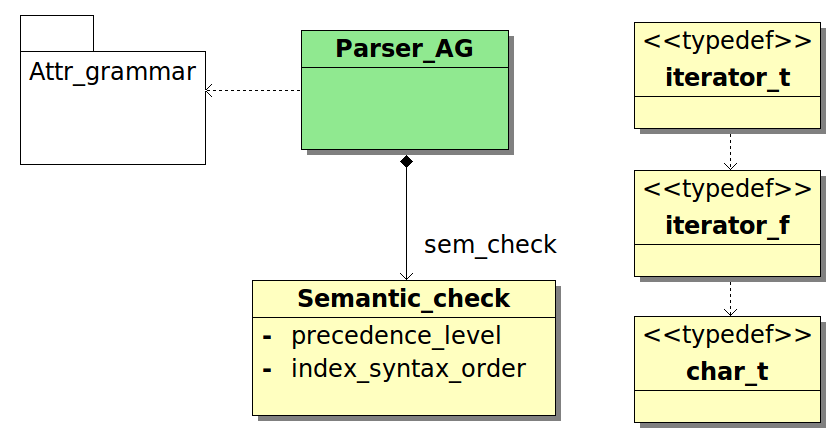
\includegraphics[width=350pt, height=184pt]{diagramas/Parser.png}
\caption{\label{fig:dia-parser}Paquete de parsing de \maggen.}
\end{figure}

\begin{figure}[!ht]\centering
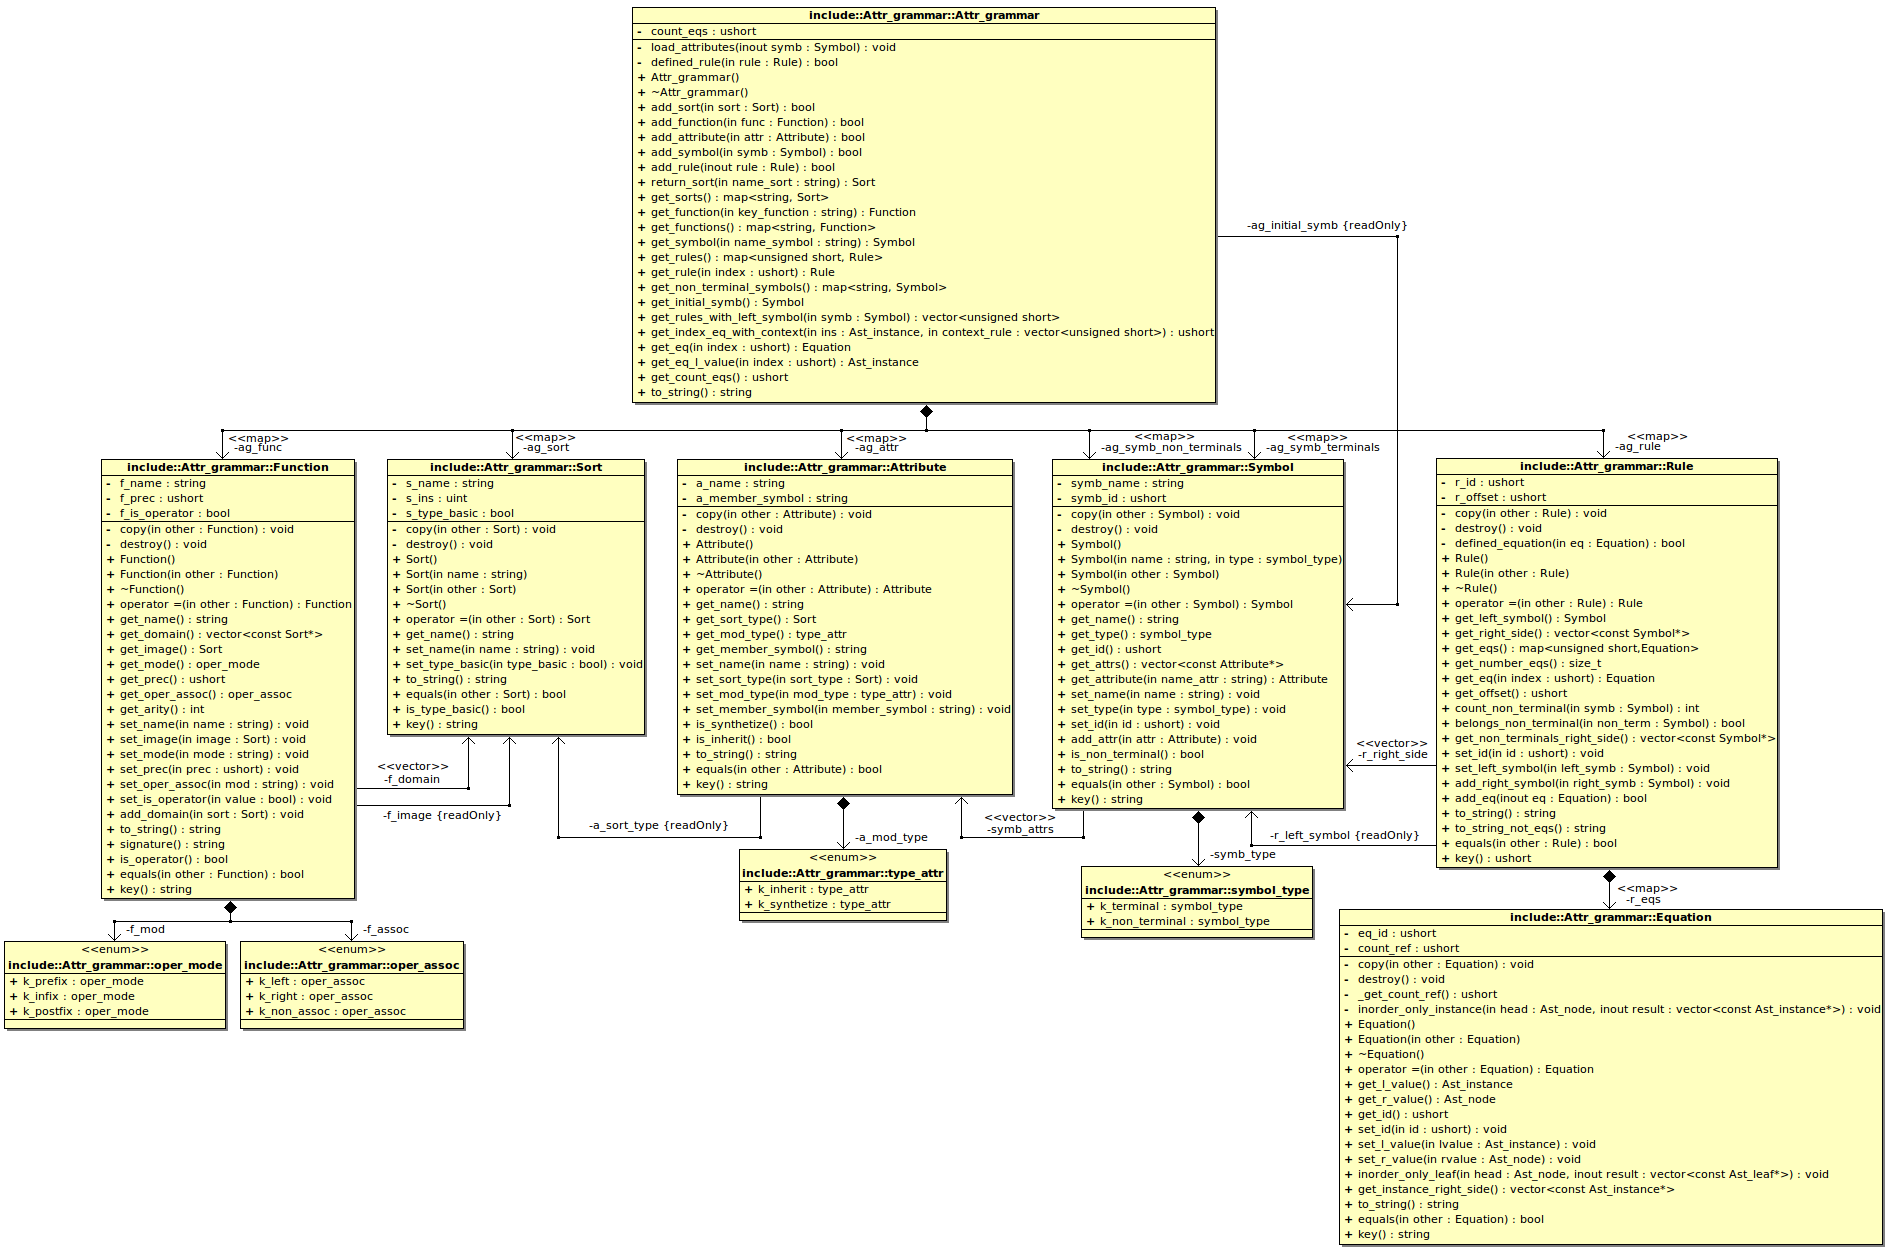
\includegraphics[width=605pt, height=300pt, angle=90]{diagramas/Attr_grammar.png}
\caption{\label{fig:dia-grammar}Paquete de representación de GA, de \maggen.}
\end{figure}

\begin{figure}[!ht]\centering
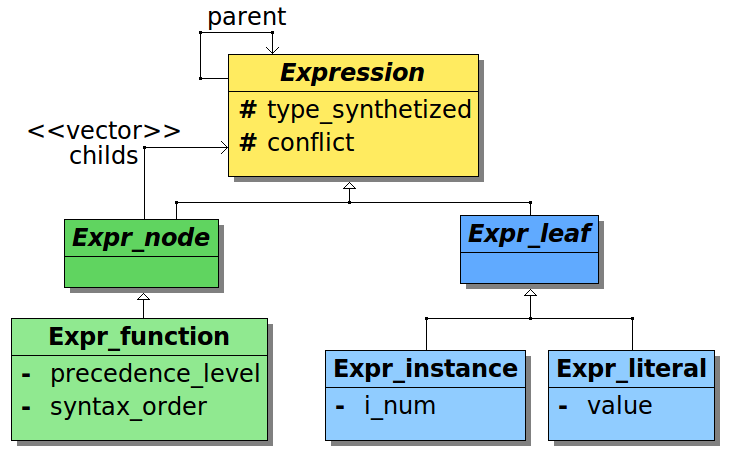
\includegraphics[width=479pt, height=300pt, angle=90]{diagramas/Expression2.png}
\caption{\label{fig:dia-express}Paquete de representación de expresiones de \maggen.}
\end{figure}

\begin{figure}[!ht]\centering
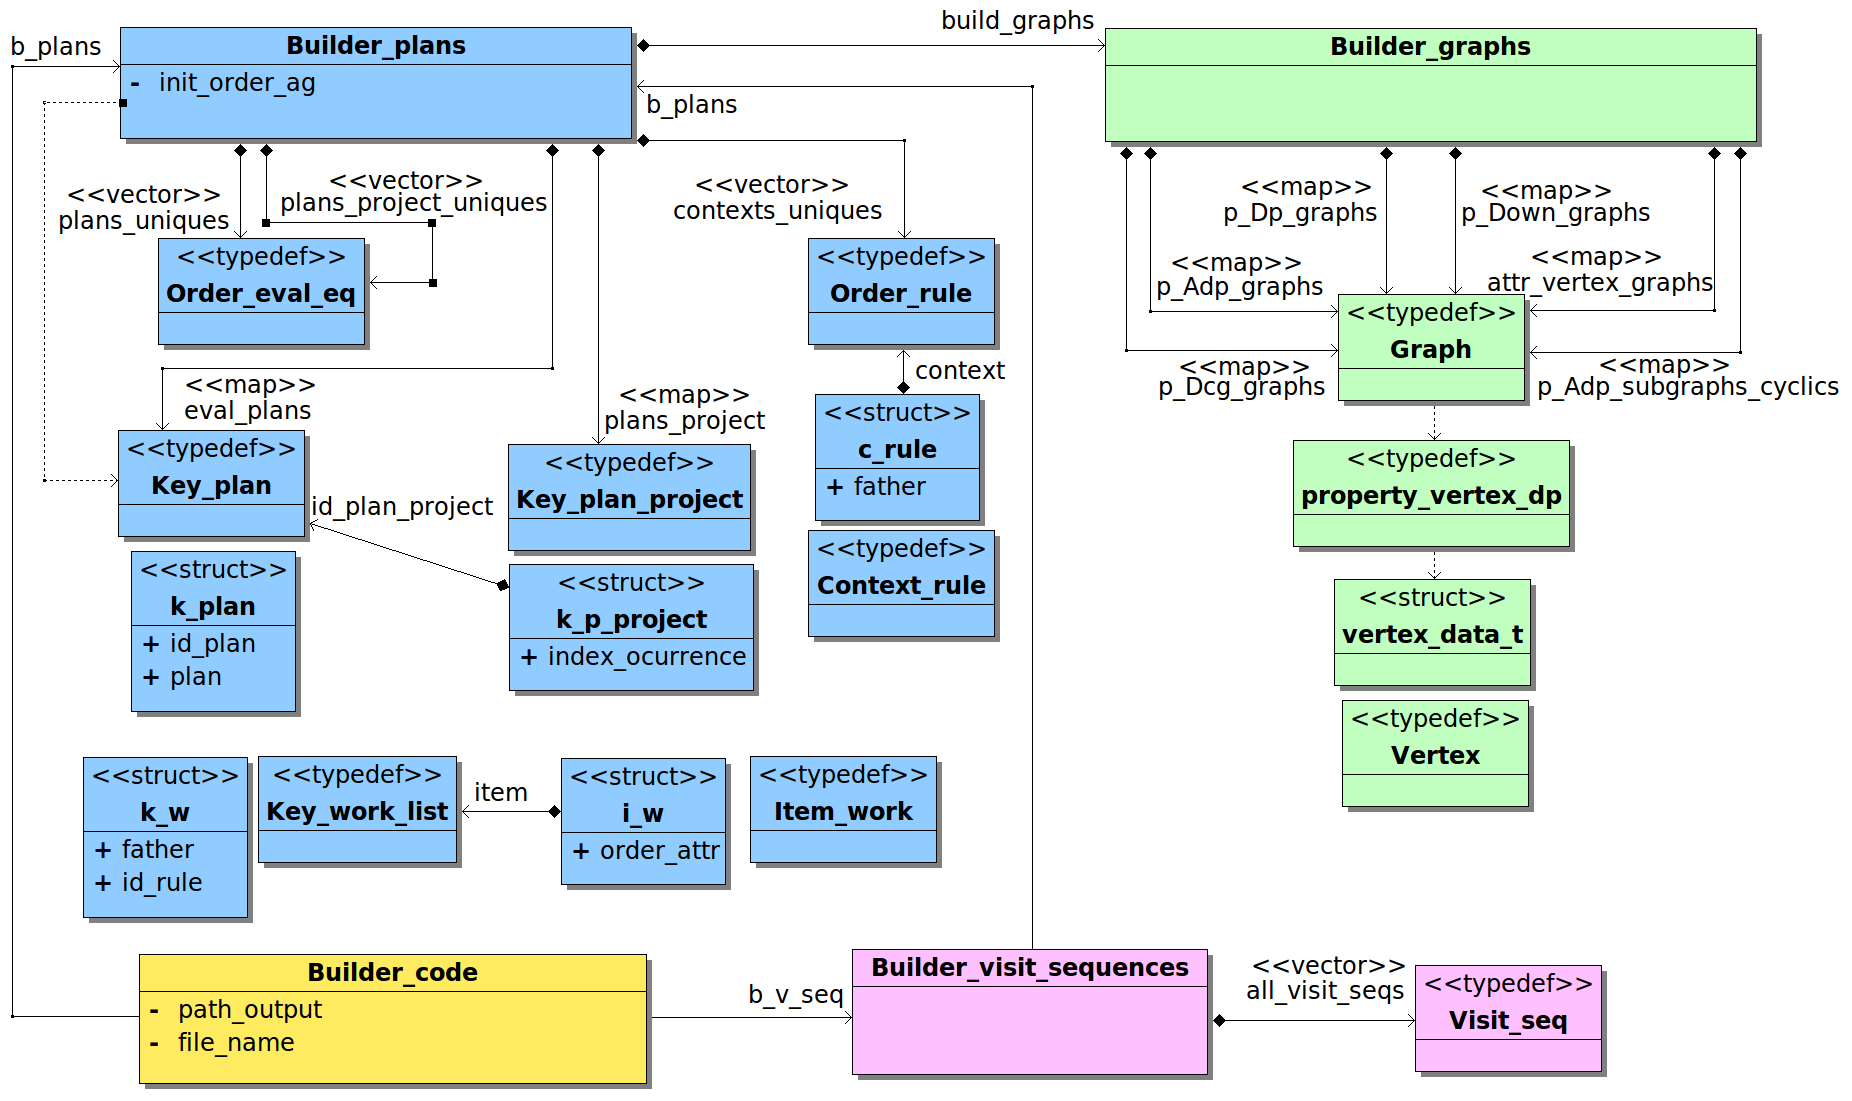
\includegraphics[width=505pt, height=300pt, angle=90]{diagramas/Builder.png}
\caption{\label{fig:dia-builders}Paquete de constructores de grafos, planes, secuencias de visita y generación código, de \maggen.}
\end{figure}

\begin{figure}[!ht]\centering
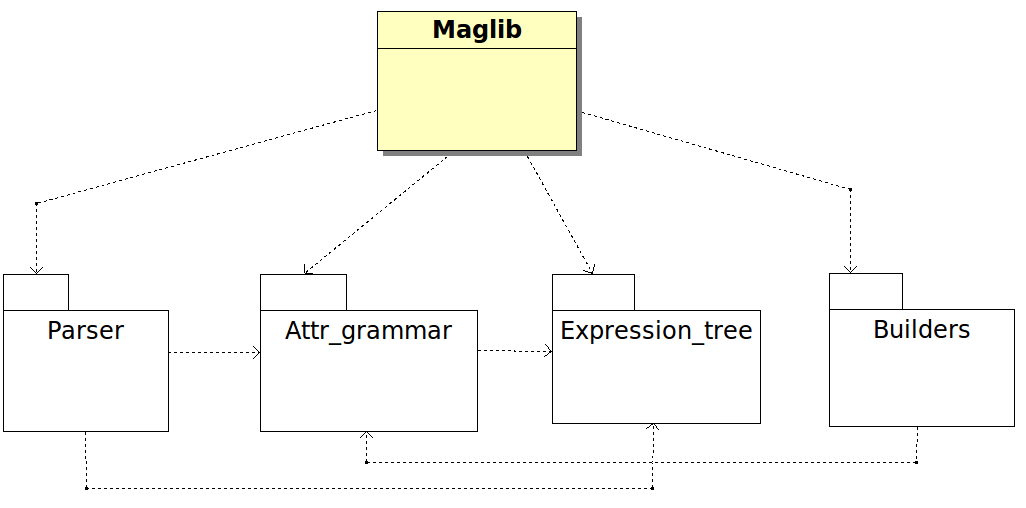
\includegraphics[width=635pt, height=300pt, angle=90]{diagramas/maggen.png}
\caption{\label{fig:dia-maglib}Paquete de libreria maglib, dentro de \maggen.}
\end{figure}

\begin{figure}[!ht]\centering
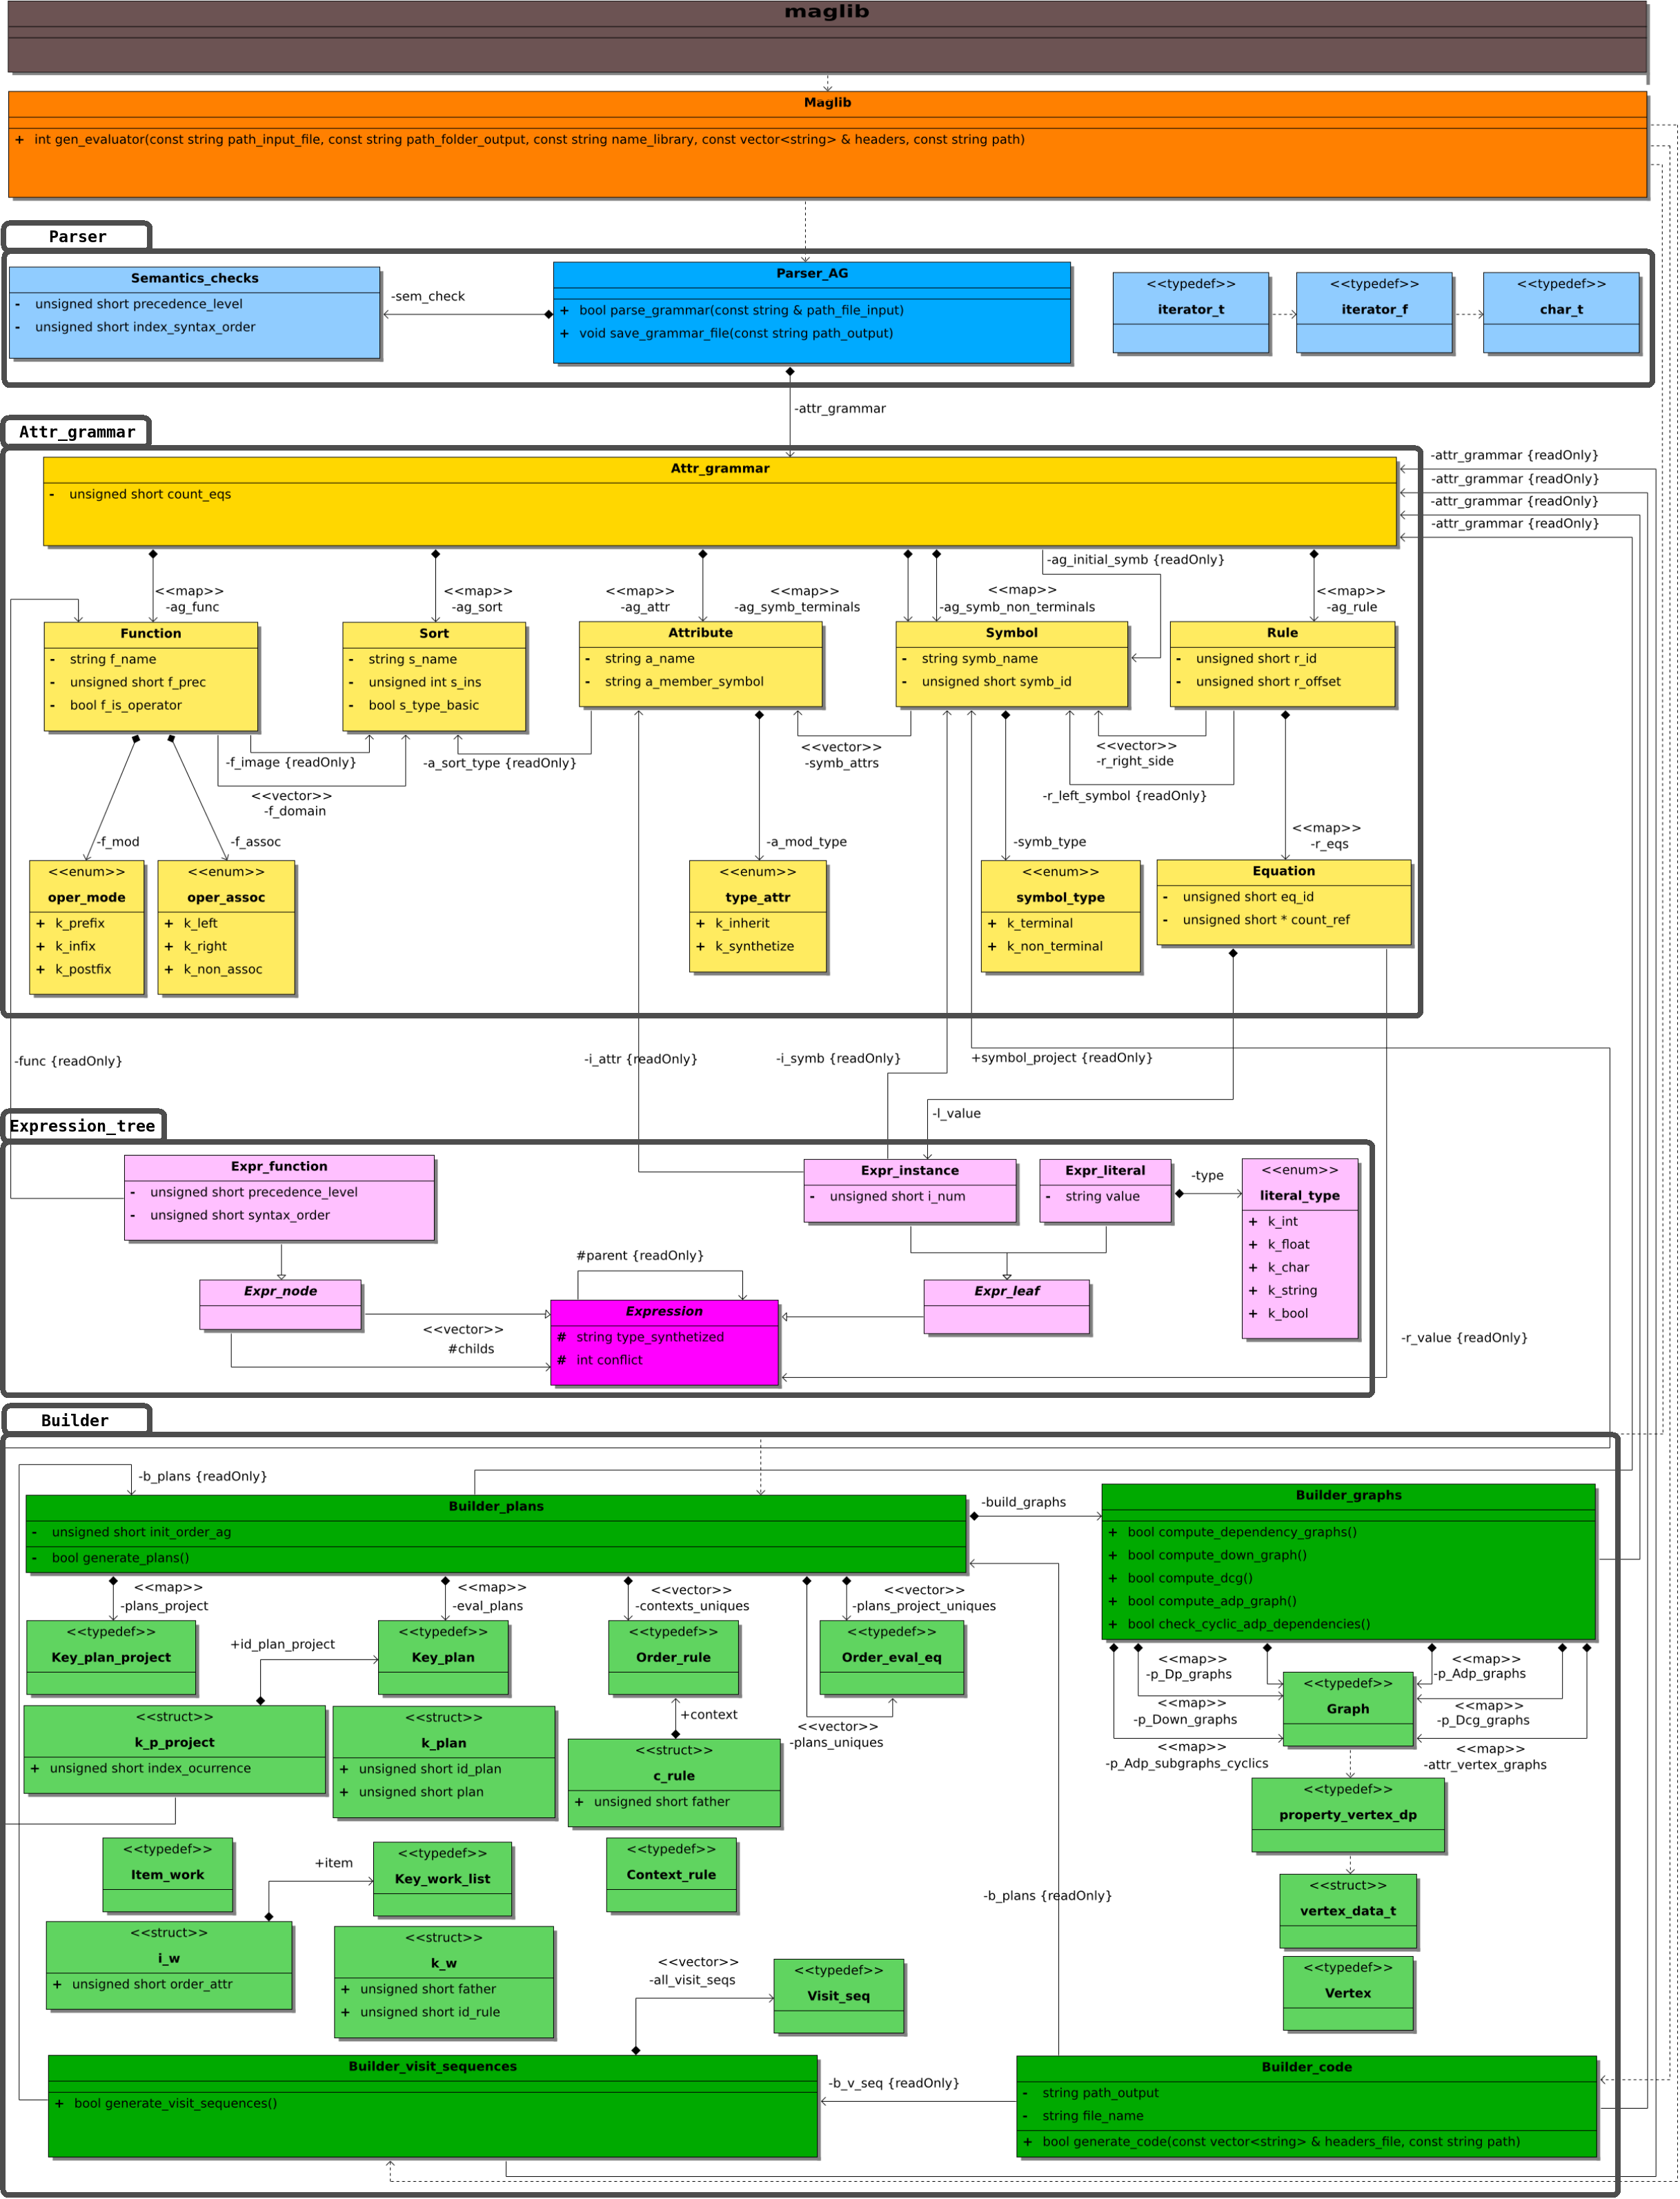
\includegraphics[width=450pt, height=589pt]{diagramas/arquitectura.png}
% 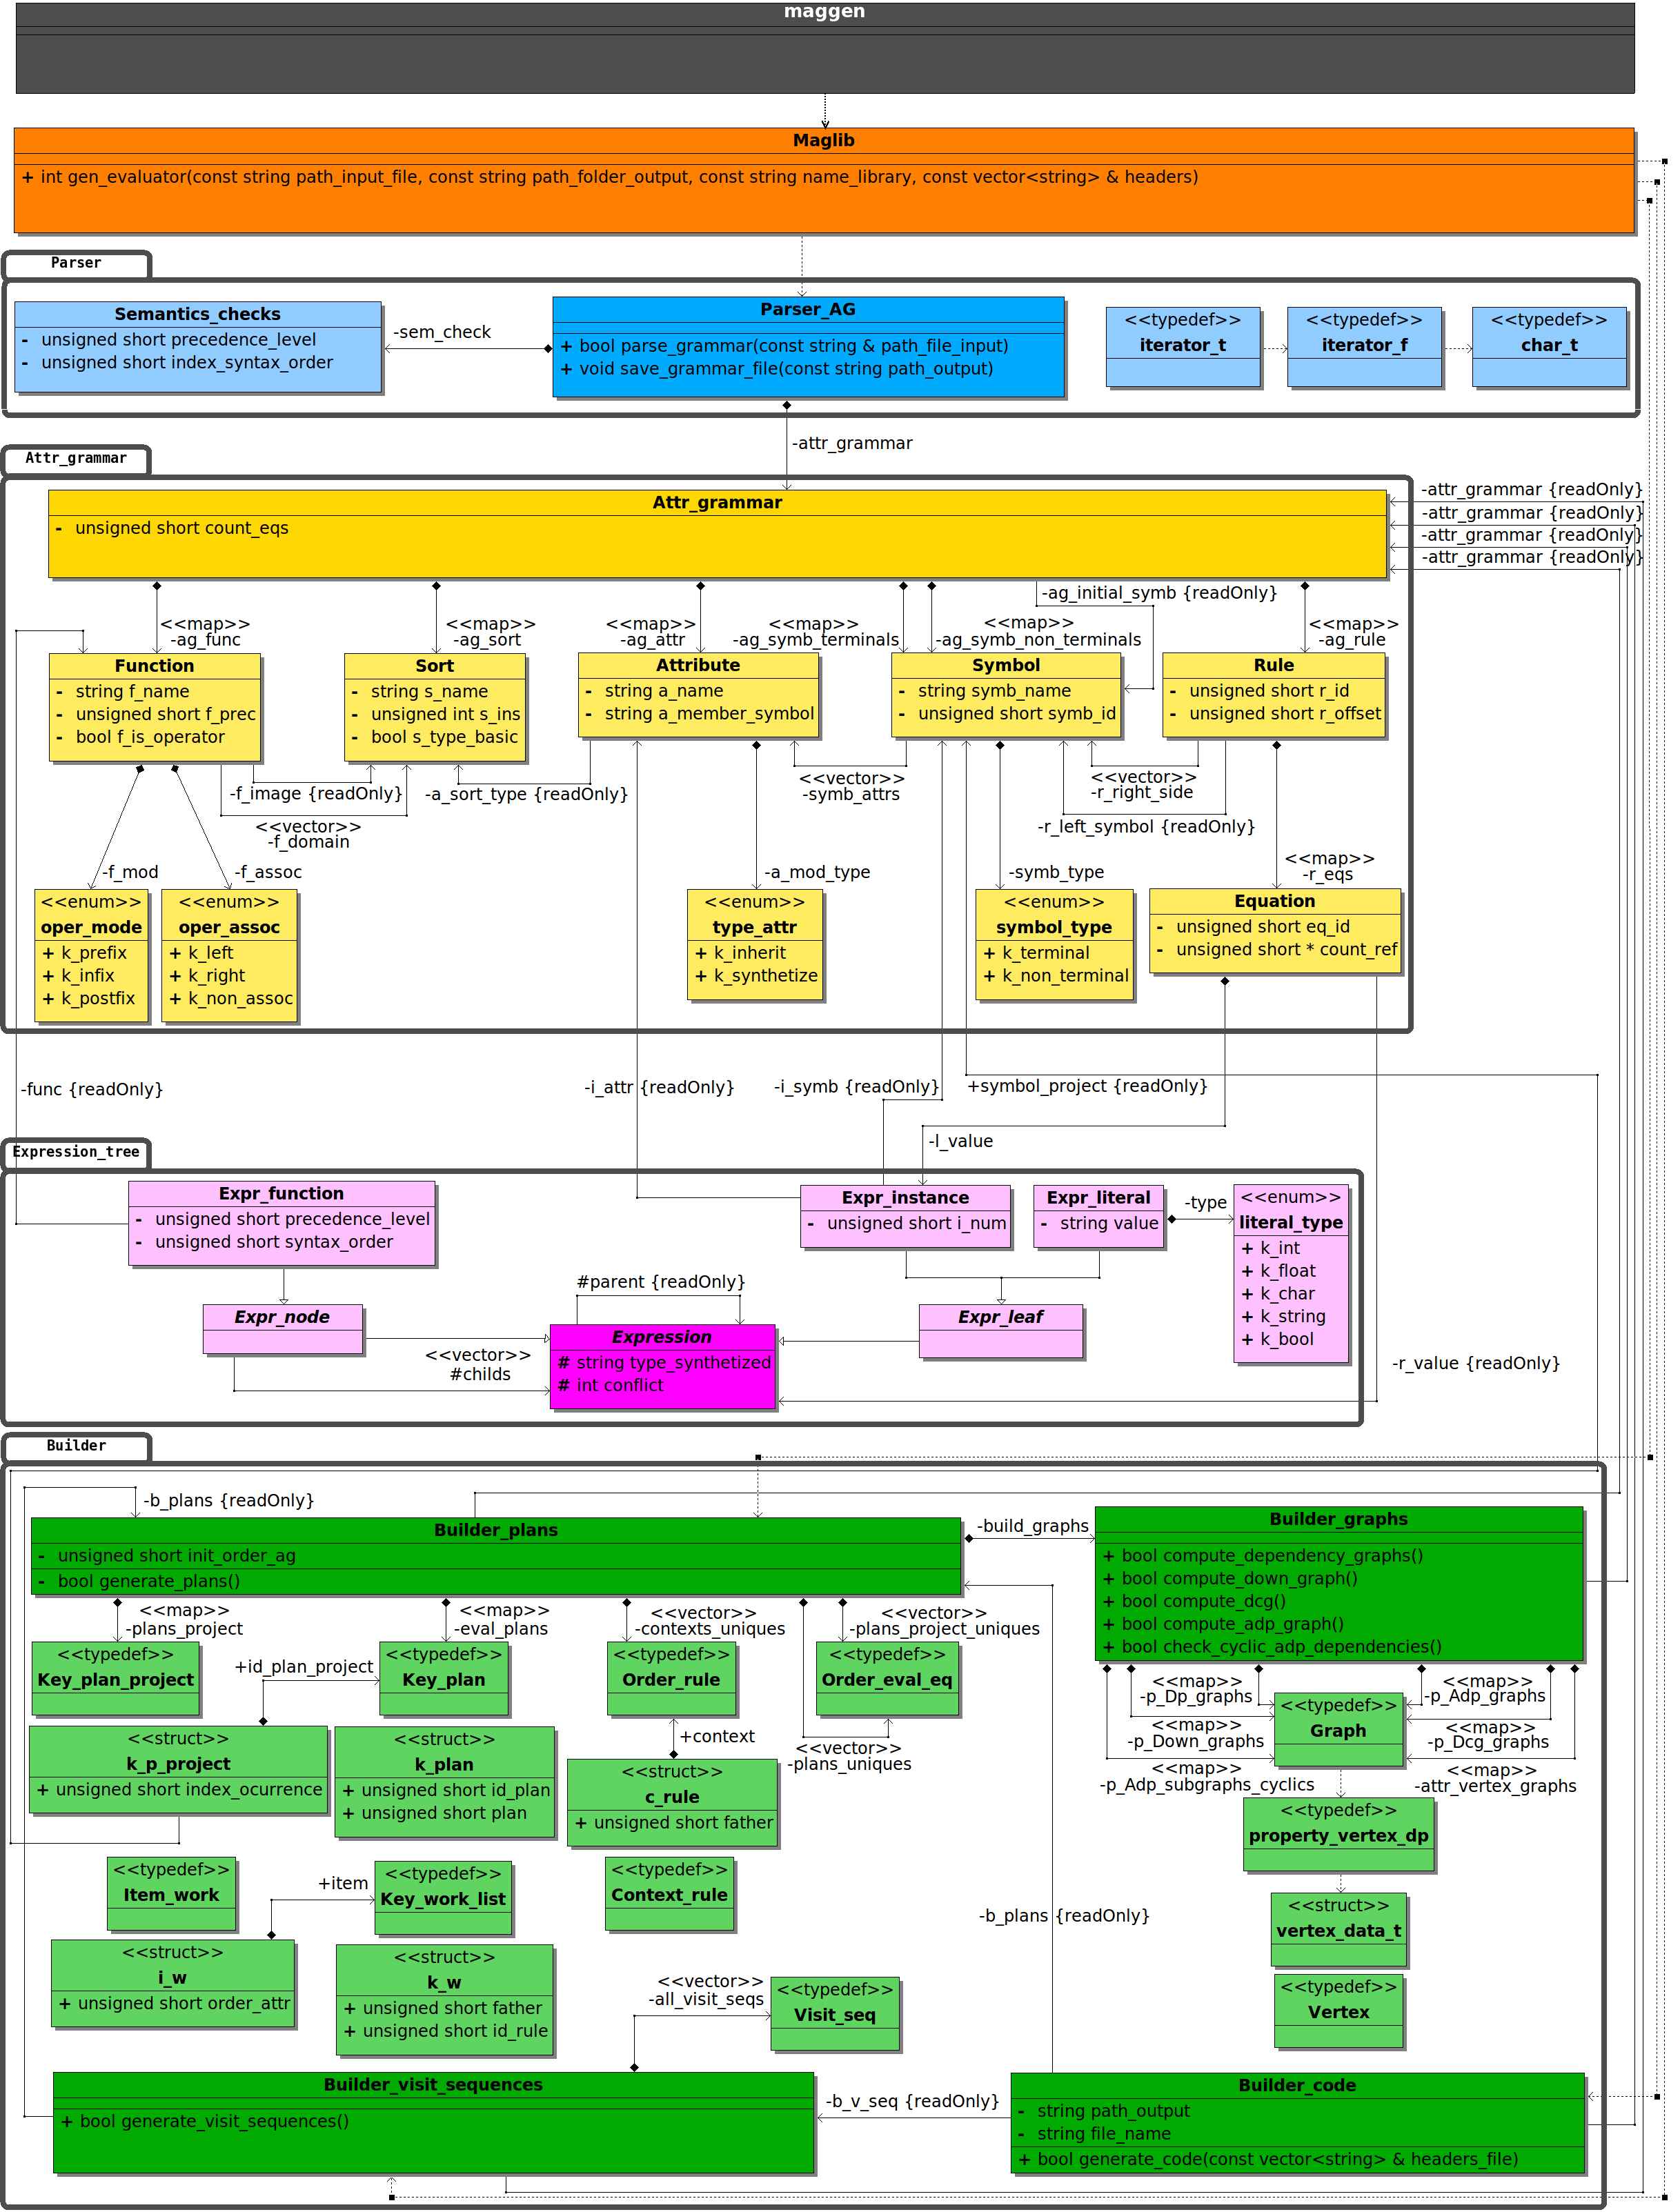
\includegraphics[width=300pt, height=395pt]{clases_full.png}
\caption{\label{fig:arquitec-full}Arquitectura completa de \maggen.}
\end{figure}



% \normalsize
\chapter{Apéndice: Documentación completa de \maggen.}
\label{chap:appendix-doxy}
La documentación completa de \maggen\ puede ser encontrada en el CD que acompaña este documento. La misma cuenta con más de 400 páginas (Documentación generada con \textit{Doxygen}), por lo que no fue conveniente incluirla en este informe. 

Además, de contar con detalles de implementación de cada clase, cuenta con diagramas auto-generados, que muestran el acoplamiento entre cada módulo.

